\documentclass[12pt]{article}
\usepackage[utf8]{inputenc}
\usepackage{amsmath,amssymb}
\usepackage{graphicx}
\usepackage{caption}
\usepackage{subcaption}

\usepackage[backend=bibtex]{biblatex}
\addbibresource{referencias.bib}

\title{Detecção de objetos }
\author{Fernando Pujaico Rivera}
\date{}

\usepackage[top=25mm, bottom=25mm, left=25mm, right=25mm]{geometry}

\usepackage{amsthm}
\newtheorem*{remark}{Remark}

\begin{document}


\maketitle


%%%%%%%%%%%%%%%%%%%%%%%%%%%%%%%%%%%%%%%%%%%%%%%%%%%%%%%%%%%%%%%%%%%%%%%%%%%%%%%%
\section{Calculando a altura $z$}
Para obter a altura $z$ de um objeto a partir de um valor $c_0$ 
extraído de uma imagem em 2D, é usada a função
$func\_z(c_0;\mathbf{K})$, 
\begin{equation}
z = func\_z(c_0;\mathbf{K}),
\end{equation}
\begin{equation}\label{eq:setupz1}
func\_z(c_0;\mathbf{K})\equiv\frac{
D~tg(\theta)
\left[
1+ ctg\left(\theta+atg\left(\frac{h_0}{d_0+c_0}\right)\right) ctg\left(\theta-atg\left(\frac{d_0}{h_0}\right)\right) 
\right]
}{
\left[1+ctg\left(\theta+atg\left(\frac{h_0}{d_0+c_0}\right)\right) \left(\frac{D~tg(\theta)ctg\left(\theta-atg\left(\frac{d_0}{h_0}\right)\right)- f}{g}\right)\right]
},
\end{equation}
sendo $\mathbf{K}=[d_0,h_0,D,\theta,f,g]^T$
um vetor que contem os parâmetros que não modificam seu valor em todos os analises,
pois pertencem à geometria do sistema implementado (setup).
Assim, se conhecemos o vetor $\mathbf{K}$, o cálculo da altura $z$, mediante a função $func\_z()$,
depende unicamente da variável $c_0$.
Porém o cálculo dos parâmetros em $\mathbf{K}$ mediante medições de alturas e ângulos
é um trabalho laborioso que traz muitos erros de medida.
Pelo que em vez de tentar obter ou medir os parâmetros em $\mathbf{K}$,
aqui se optou por realizar a seguinte aproximação da função $func\_z()$, 
mediante a função $f_{\mathbf{P}}()$, 
\begin{equation}
func\_z(c_0;\mathbf{K})\equiv f_{\mathbf{P}}(c_0),
\end{equation}
que representa una serie de Taylor,
\begin{equation}
\begin{align*}
f_{\mathbf{P}}(c_0)  &\equiv p_0+p_1~c_0+p_2~c_0^2+p_3~c_0^3+...\\ 
 &\equiv \sum_{i=0}^{\infty}p_i~c_0^i
\end{align*}
\end{equation}
na qual, o vetor $\mathbf{P}=[p_0,~p_1,~p_2,~...]$ tem infinitos elementos. 
O parâmetro $p_0$ é fácil de aproximar pois se assume que $f_{\mathbf{P}}(0)\approx 0$,
de modo que $p_0\approx 0$ e 
\begin{equation}
f_{\mathbf{P}}(x)  \equiv p_1~x+p_2~x^2+p_3~x^3+...
\end{equation}
a partir de aqui realizamos uma aproximação considerando a geometria do sistema
e testes para identificar o erro desta aproximação. Finalmente foi observado
que um polinômio de primeiro ordem (quer dizer $p_i=0|\forall i\geq 2$) 
já produzia uma aproximação adequada à altura real dos objetos,
pelo que agora  
\begin{equation}
func\_z(c_0;\mathbf{K})\equiv f_{\mathbf{P}}(c_0)\approx p_1 c_0;
\end{equation}
assim, o único parâmetro desconhecido é $p_1$.
\begin{remark}
É importante ressaltar que esta é uma aproximação,
pelo que se houvéssemos escolhido
$func\_z(c_0;\mathbf{K}) \approx p_0 + p_1 c_0+p_2 c_0^2$,
poderíamos ter atingido reconstruções mais apuradas,
porém a aproximação de primeiro ordem já cumpre com o objetivo.
\end{remark}

Assim, usando a função $f_{\mathbf{P}}(c_0)$ podemos achar a altura $z$
a partir do valor $c_0$ numa fotografia, como mostra a Figura \ref{fig:setup1}.
Lembrando que $c_0$ é a medida de diferencia da altura entre de um objeto na fotografia
e a linha de referencia numa posição $d_0$.
\begin{figure}[!h]
     \centering
         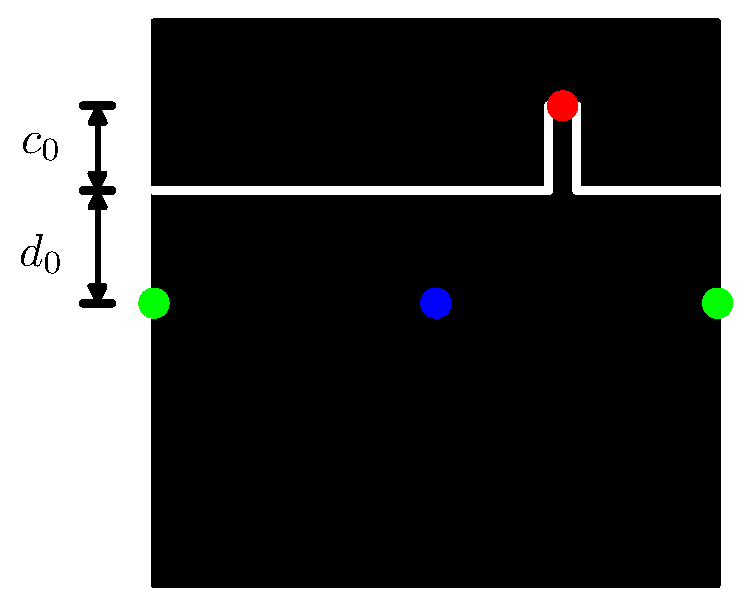
\includegraphics[width=0.7\textwidth]{Diagrama7.eps}
\caption{Obtendo o valor $c_0$.}
\label{fig:setup1}
\end{figure}

Por outro lado, para obter o valor $p_1$ é usado um objeto de tamanho $z$ conhecido,
ao qual se lhe toma uma fotografia e se obtém o valor $c_0$;
assim, para obter o valor $p_1$ usamos,
\begin{equation}
p_1=\frac{z}{c_0}.
\end{equation}
\begin{remark}
Para aprimorar mais o cálculo de $p_1$ também poderiam ser tomadas varias amostras
$d_n=\{z^{(n)},c_0^{(n)}\}$, para todo inteiro $n$ que cumpra $1\leq n \leq N$.
De modo que $p_1=E\left[\frac{z^{(n)}}{c_0^{(n)}}\right]$, 
sendo que $E[.]$ representa ao operador esperança.
\end{remark}


\printbibliography
\end{document}
